
\documentclass[openany,11pt]{homework}

\coursename{ELEN 4903 Machine Learning (Spring 2018)} % DON'T CHANGE THIS

\studname{Pratyus Pati}    % YOUR NAME GOES HERE
\studmail{pp2636@columbia.edu}% YOUR UNI GOES HERE
\hwNo{4}                   % THE HOMEWORK NUMBER GOES HERE

% Uncomment the next line if you want to use \includegraphics.
\usepackage{graphicx}

\begin{document}
\maketitle

\section*{Problem 1(a)}

\begin{center}
	\centering
	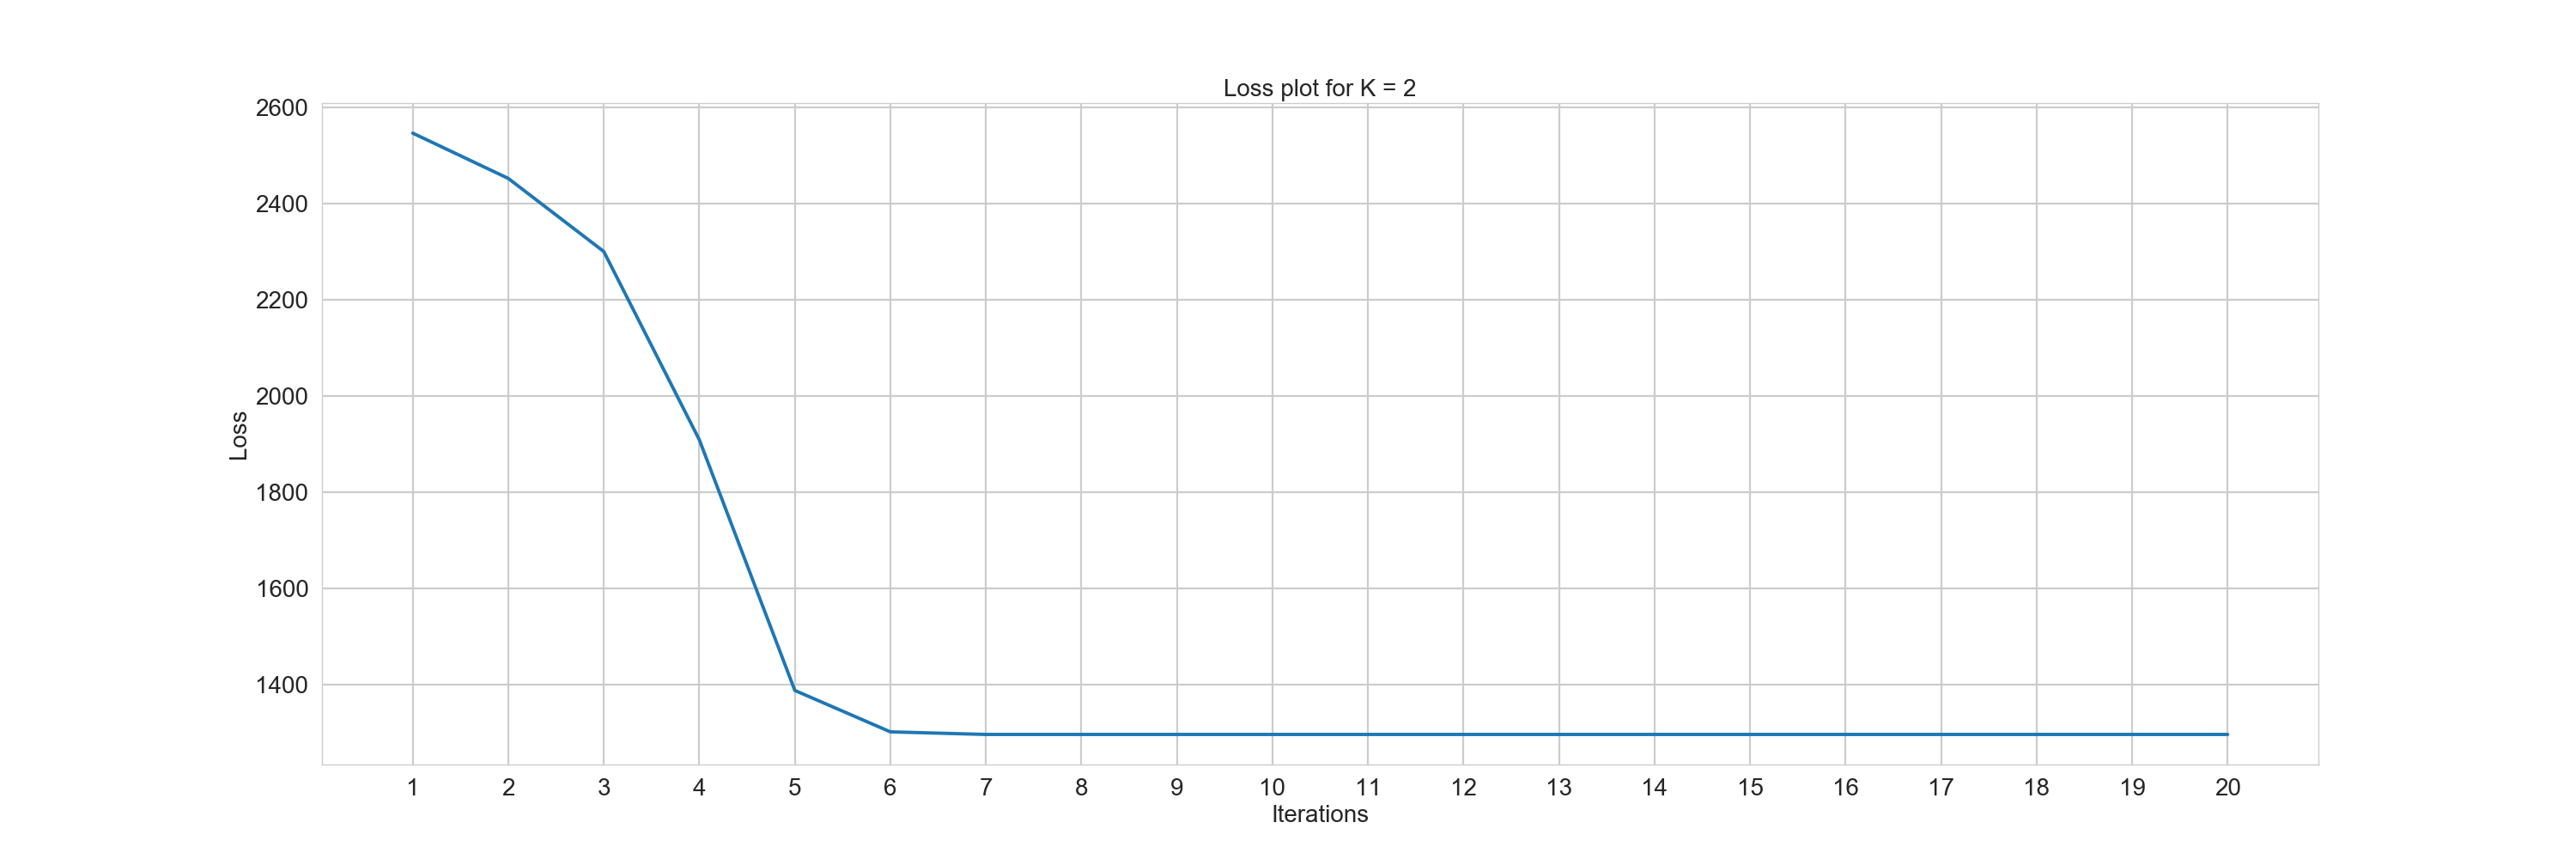
\includegraphics[width = \textwidth]{1a_2.png}
	\textbf{Loss vs. Iterations for K$=2$}
\end{center}

\begin{center}
	\centering
	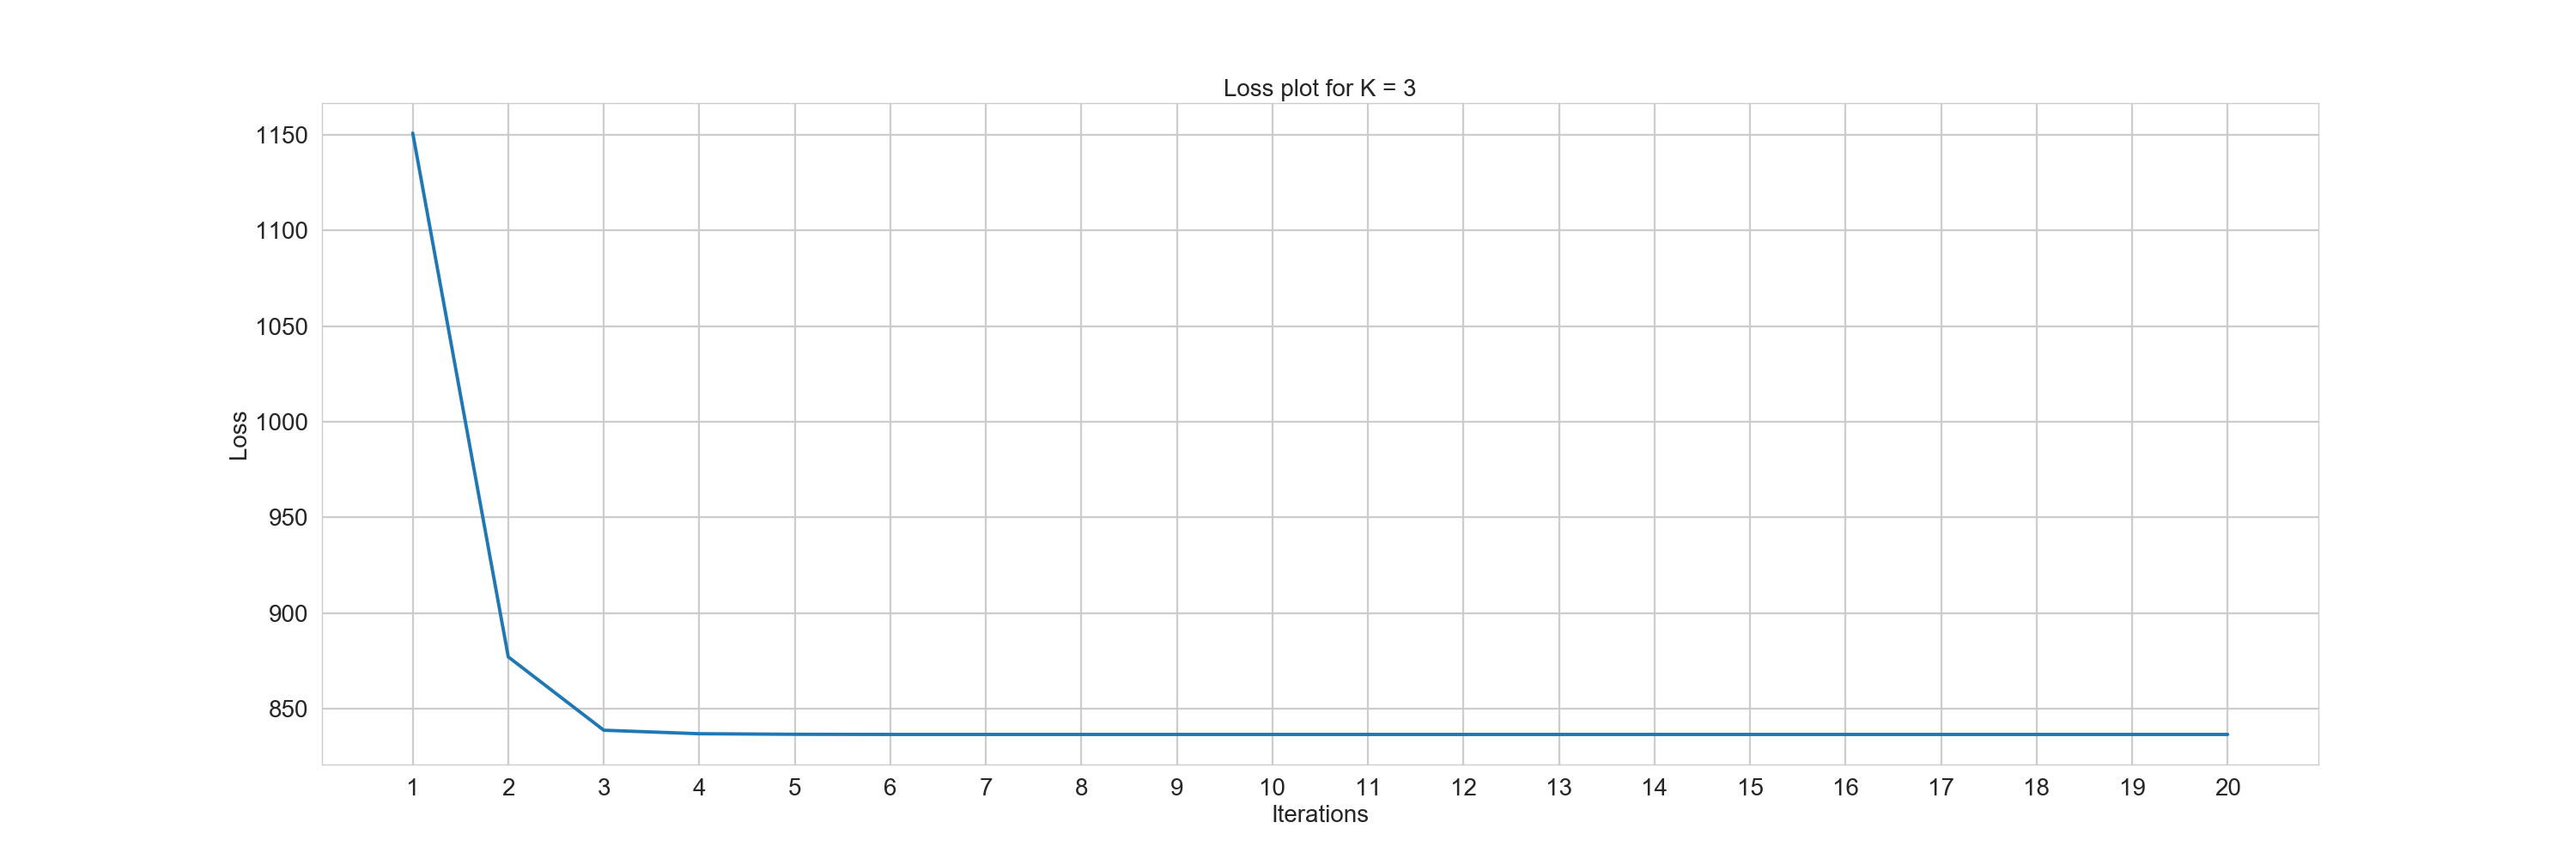
\includegraphics[width = \textwidth]{1a_3.png}
	\textbf{Loss vs. Iterations for K$=3$}
\end{center}

\begin{center}
	\centering
	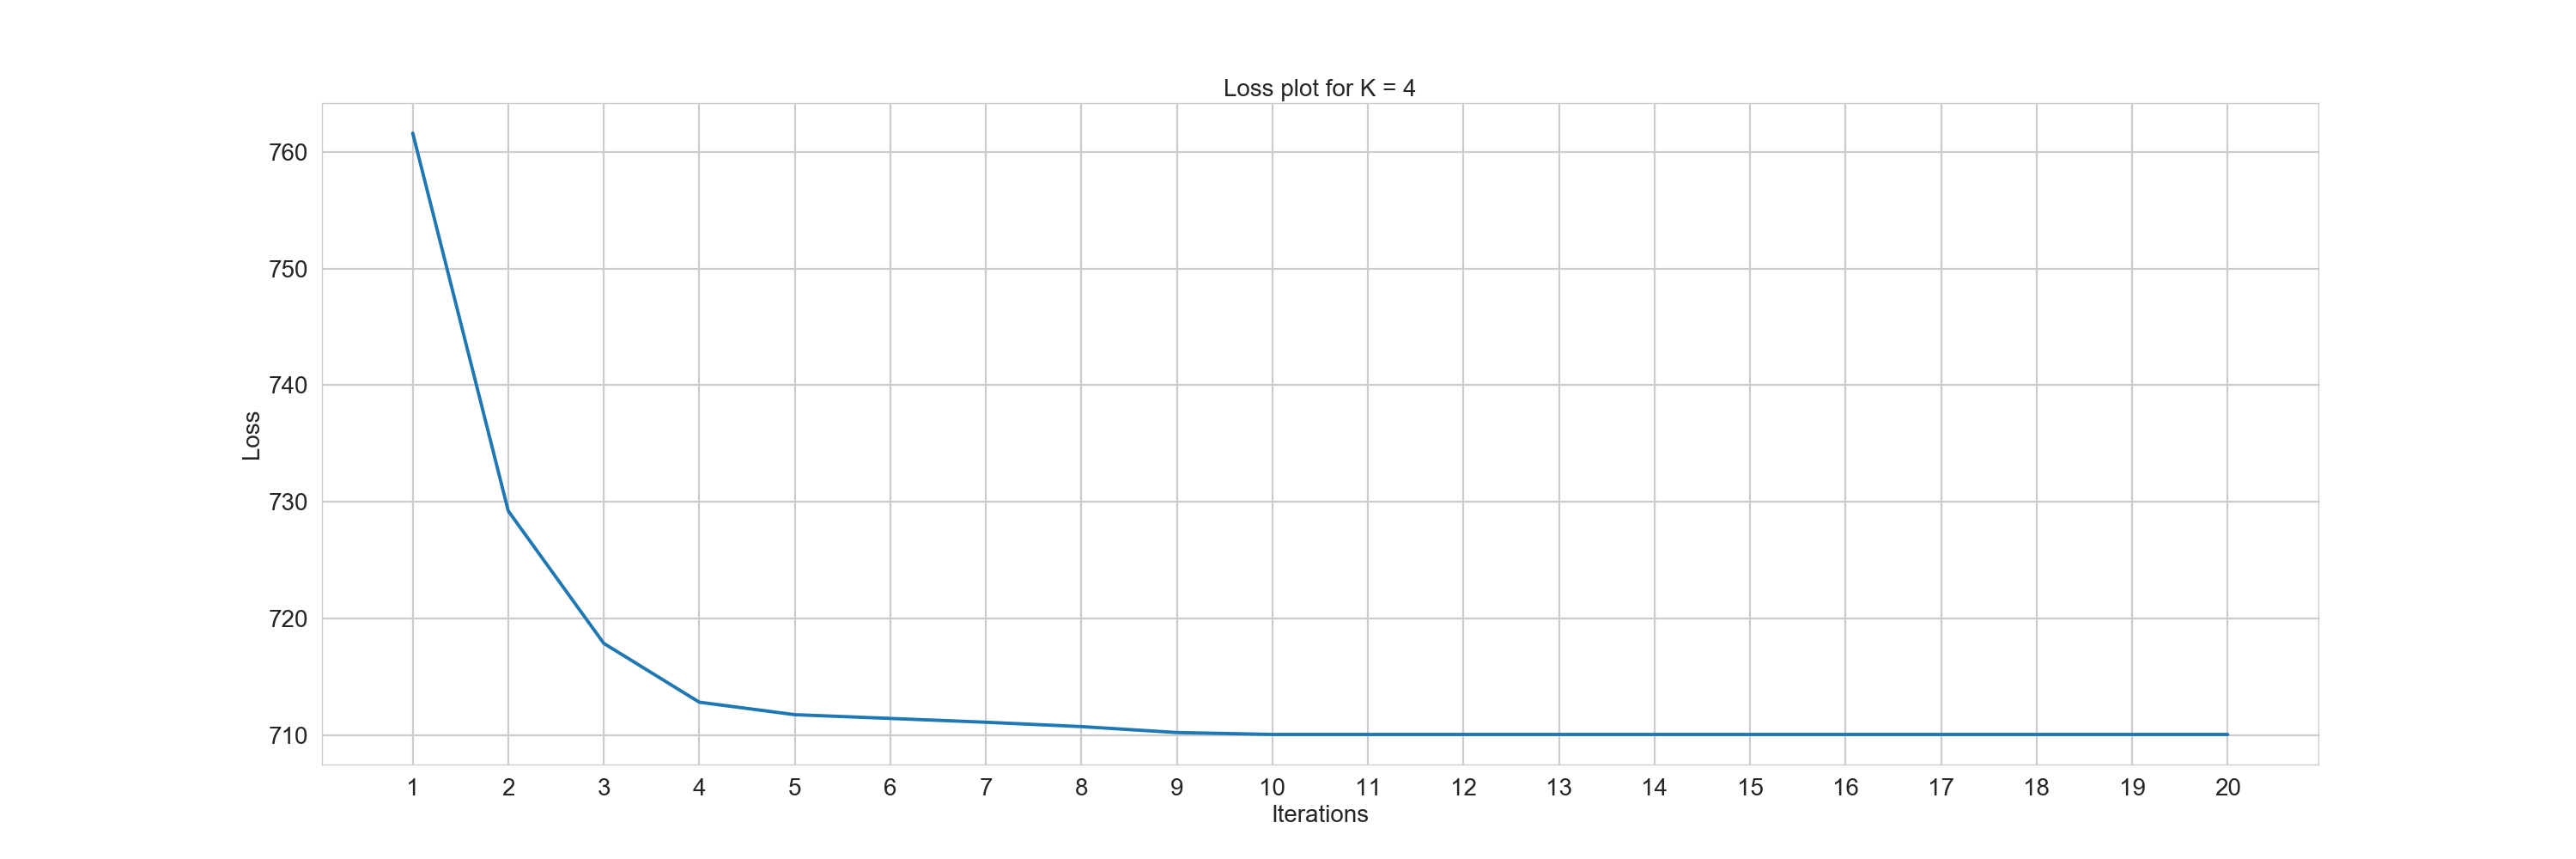
\includegraphics[width = \textwidth]{1a_4.png}
	\textbf{Loss vs. Iterations for K$=4$}
\end{center}

\begin{center}
	\centering
	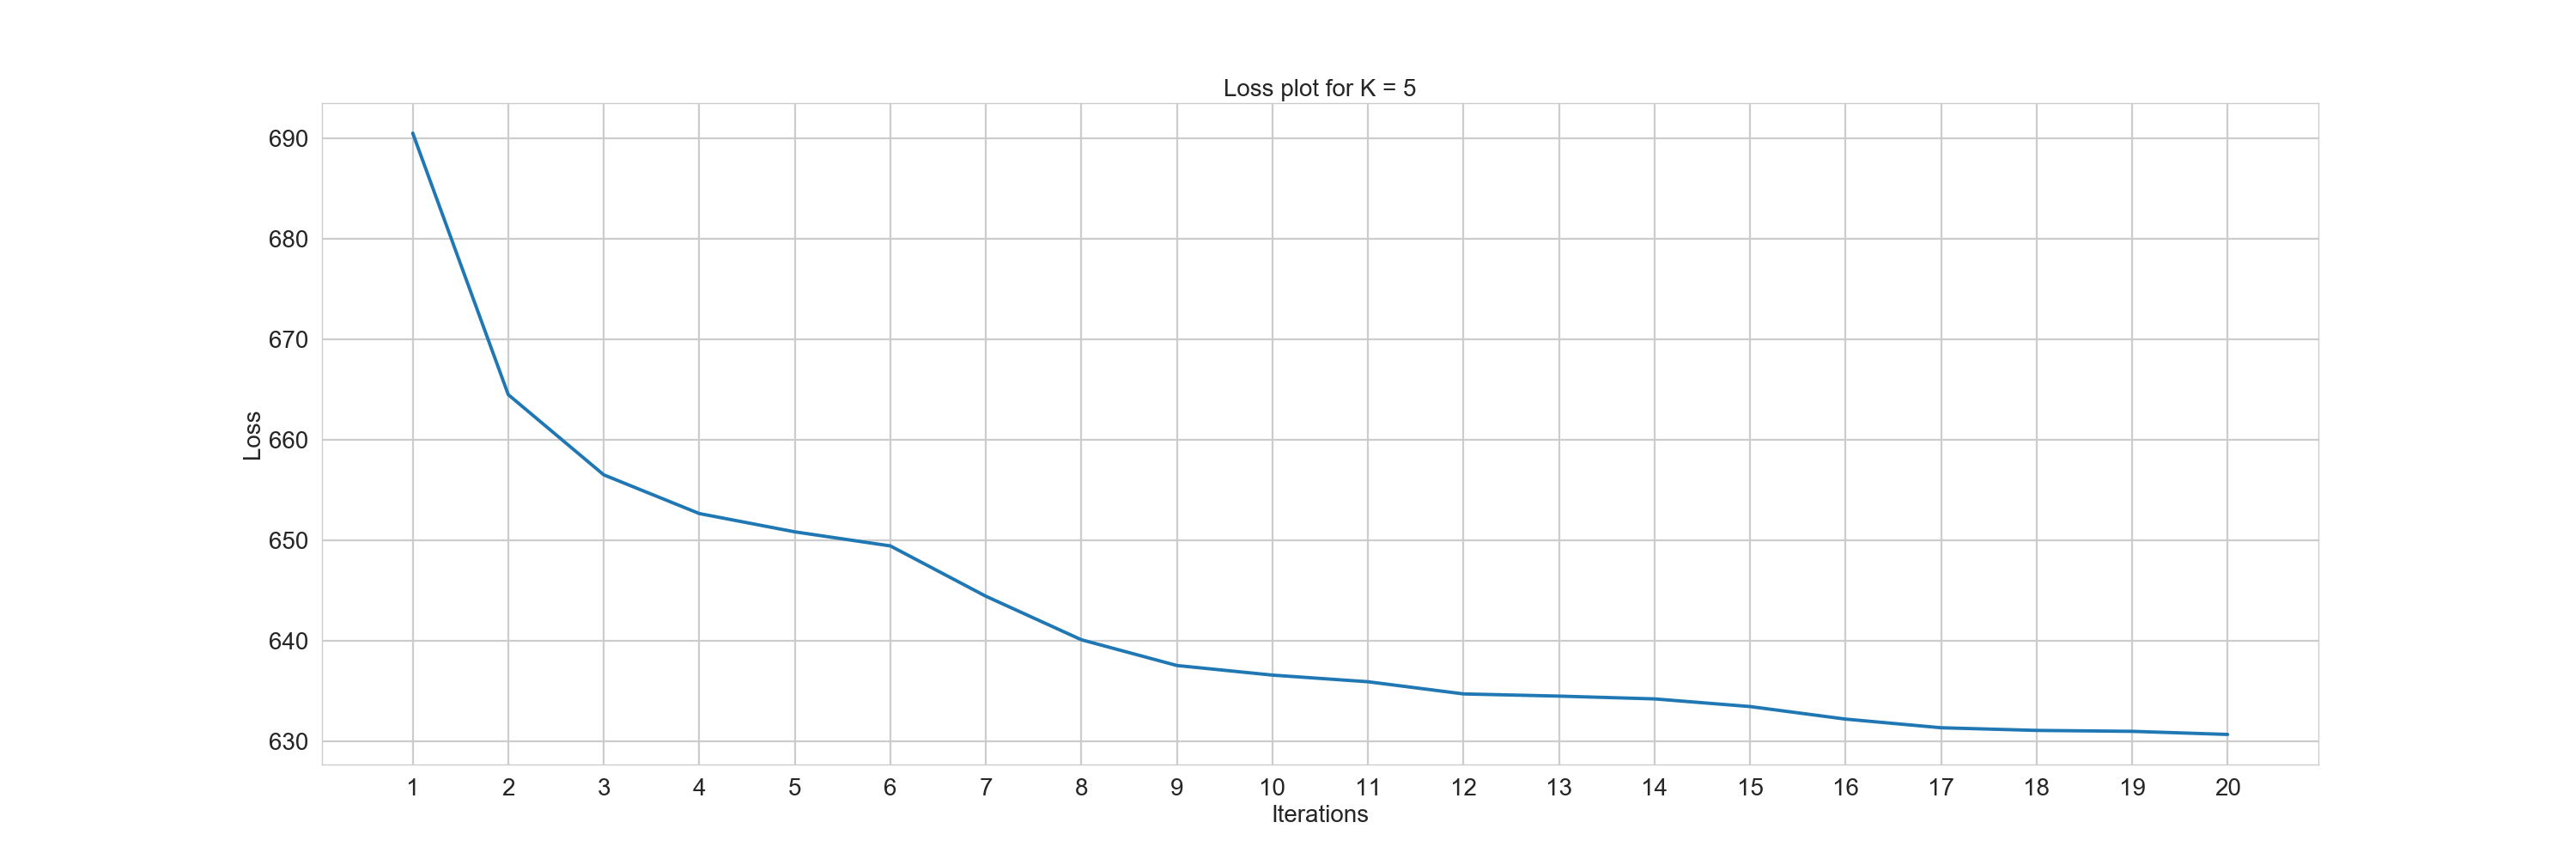
\includegraphics[width = \textwidth]{1a_5.png}
	\textbf{Loss vs. Iterations for K$=5$}
\end{center}


\section*{Problem 1(b)}
\begin{center}
	\centering
	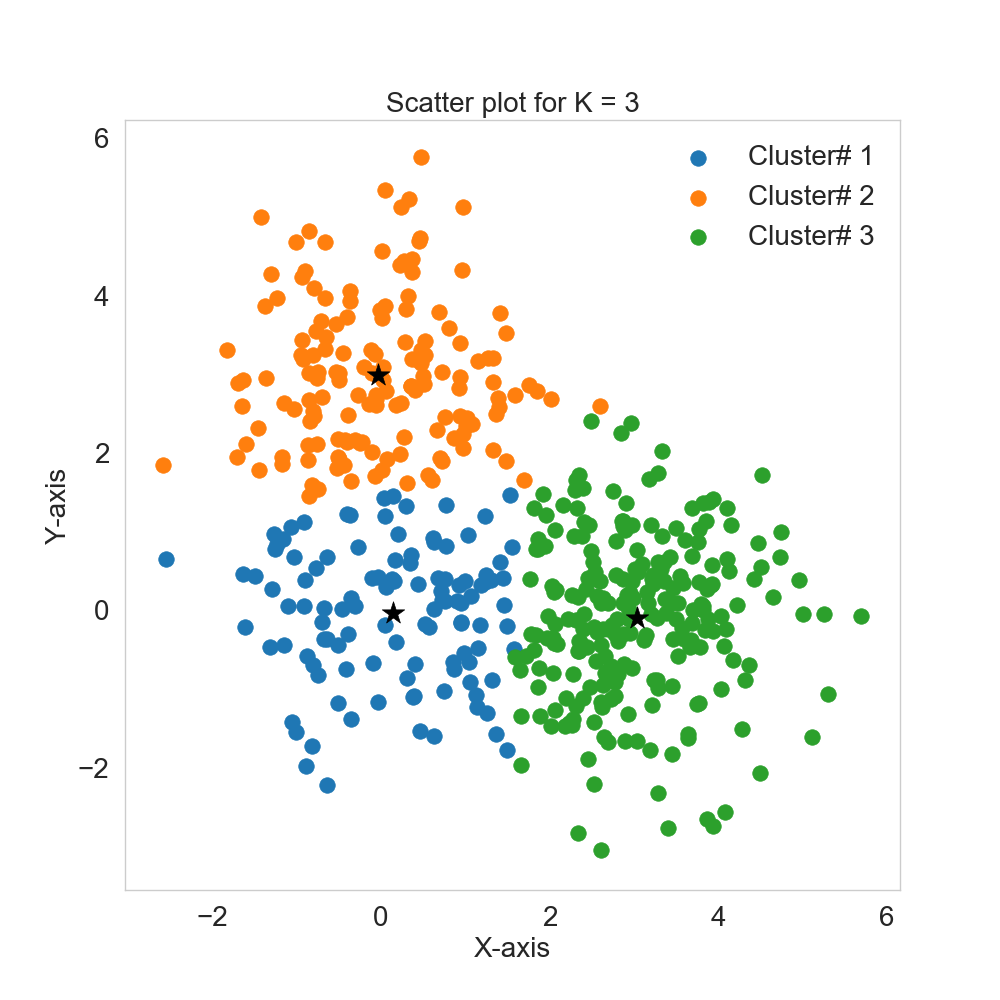
\includegraphics[width = \textwidth]{1b_3.png}
	\textbf{Cluster Scatter Plot for K$=3$}
\end{center}

\begin{center}
	\centering
	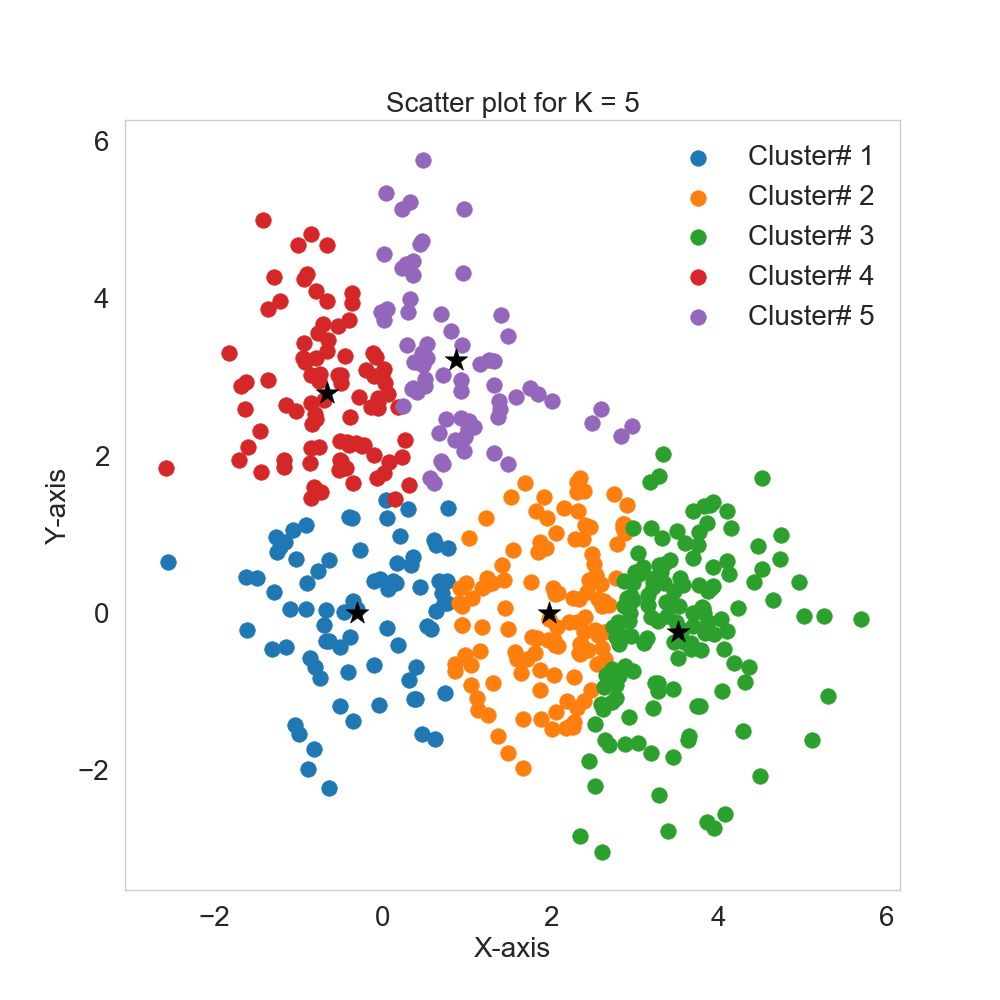
\includegraphics[width = \textwidth]{1b_5.png}
	\textbf{Cluster Scatter Plot for K$=5$}
\end{center}


\section*{Problem 2(a)}

\begin{center}
	\centering
	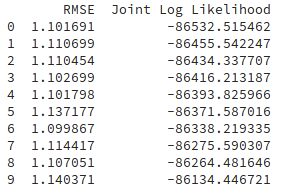
\includegraphics[width = 0.75\textwidth]{rmse_vs_jll.png}
	\textbf{RMSE vs. Joint Log Likelihood (sorted by Joint Log Likelihood)}
\end{center}

\begin{center}
	\centering
	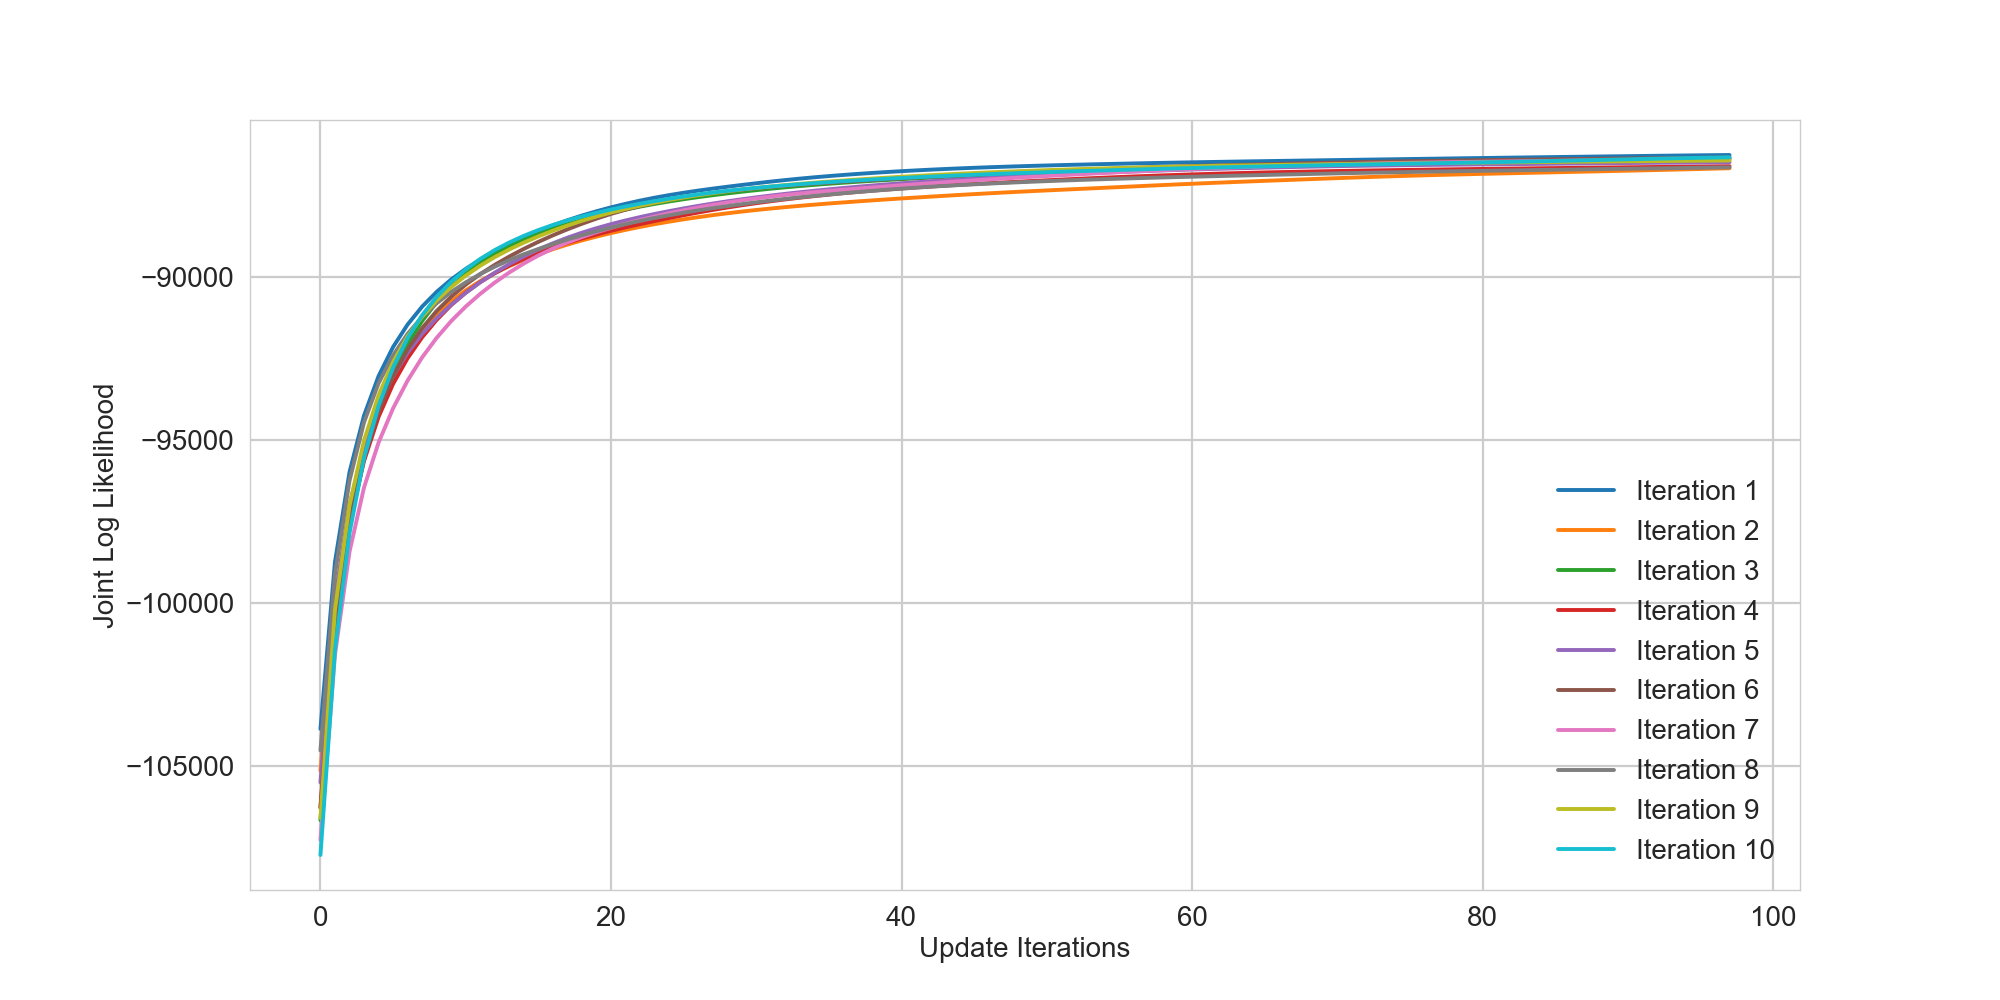
\includegraphics[width = \textwidth]{2a.png}
	\textbf{Increase of Joint Log Likelihoof over multiple iterations}
\end{center}

\newpage

\section*{Problem 2(b)}

\begin{center}
	\centering
	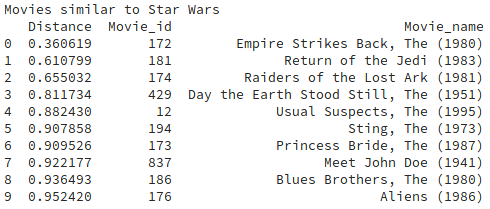
\includegraphics[width = \textwidth]{sw.png}
	\textbf{Movies similar to Star Wars}
\end{center}

\begin{center}
	\centering
	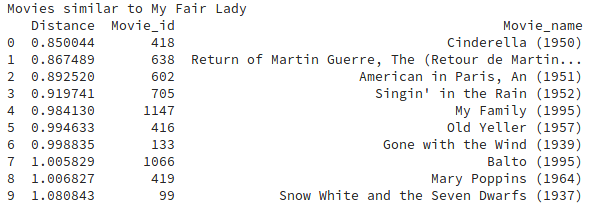
\includegraphics[width = \textwidth]{mfl.png}
	\textbf{Movies similar to My Fair Lady}
\end{center}

\begin{center}
	\centering
	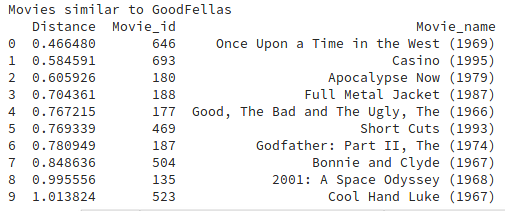
\includegraphics[width = \textwidth]{gf.png}
	\textbf{Movies similar to Goodfellas}
\end{center}

\end{document}
